\section{Results}
\label{sec:results}

\begin{figure}[t]
    \centering
    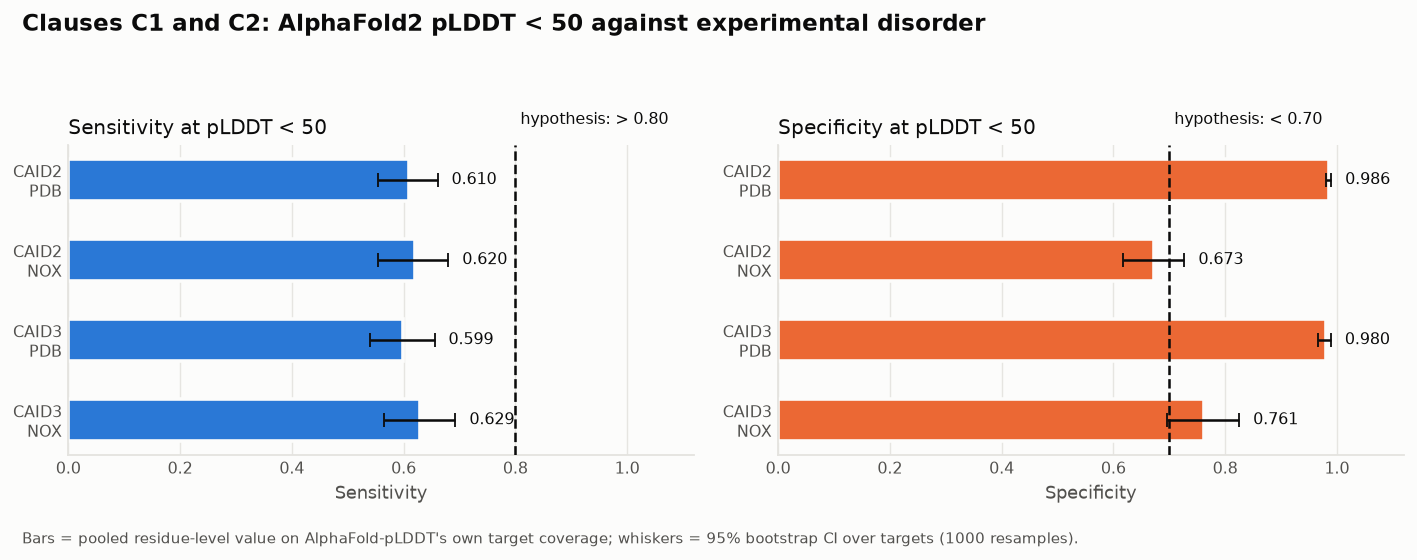
\includegraphics[width=0.95\linewidth]{figures/fig1_clause_verdict.png}
    \caption{Verdicts on the four clauses. Sensitivity of \plddtrule sits at 0.60--0.63 on every
    reference set, far below the claimed 0.8 (dashed line), and restricting to regions longer
    than 30 aa moves it only to 0.63--0.65. Specificity, at the identical operating point,
    is 0.98 under \dpdb and 0.67--0.76 under \dnox: the claim ``specificity $<$ 0.7'' is a
    property of the negative-set convention, not of AlphaFold. Error bars are 95\% bootstrap
    intervals over targets.}
    \label{fig:clause}
\end{figure}

\subsection{C1: sensitivity at \texorpdfstring{\plddtrule}{pLDDT<50} is 0.6, not 0.8}
\label{sec:c1}

\tabref{tab:clause} gives the headline numbers. Sensitivity of the literal rule is
$0.599$--$0.629$ over all disordered residues and $0.630$--$0.648$ restricted to regions longer
than 30 aa. Not one bootstrap resample out of 1000 reached sensitivity 0.80, in any of the four
settings, under either measurement: $P(\text{sens} \ge 0.80) = 0.000$ throughout. The clause
fails by roughly $0.17$ in absolute terms, an order of magnitude larger than the CI half-width.

\begin{table}[t]
    \centering
    \small
    \resizebox{\textwidth}{!}{%
    \begin{tabular}{@{}lrrllrr@{}}
        \toprule
        \textbf{Reference set} & \textbf{$n$} & \textbf{Content} &
        \textbf{Sensitivity (95\% CI)} & \textbf{Sens.\ $>$30 aa} &
        \textbf{Specificity} & \multicolumn{1}{c}{$P(\text{sens}\!\ge\!0.8)$} \\
        \midrule
        \caidtwo \dpdb   & 299 & 0.299 & 0.610 [0.554, 0.661] & 0.634 [0.573, 0.687] & \textbf{0.986} & 0.000 \\
        \caidtwo \dnox   & 173 & 0.235 & 0.620 [0.553, 0.680] & 0.630 [0.562, 0.693] & 0.673 & 0.000 \\
        \caidthree \dpdb & 319 & 0.316 & 0.599 [0.540, 0.655] & 0.630 [0.564, 0.691] & \textbf{0.980} & 0.000 \\
        \caidthree \dnox & 204 & 0.264 & 0.629 [0.565, 0.693] & 0.648 [0.580, 0.711] & 0.761 & 0.000 \\
        \bottomrule
    \end{tabular}}
    \caption{Clause tests for \plddtrule on \plddt's own target coverage. ``Content'' is the
    fraction of evaluated residues that are disordered. Specificity 95\% CIs are
    [0.981, 0.990], [0.618, 0.727], [0.966, 0.989] and [0.696, 0.825] respectively.
    Sensitivity never approaches 0.8; specificity is decided by the reference convention.}
    \label{tab:clause}
\end{table}

\para{The result is not an artefact of the target set.} Sensitivity ranges over $0.51$--$0.63$
across three target-set conventions --- the full-panel intersection, \plddt's own coverage, and
the full reference with AlphaFold's 49 missing \caidtwo targets scored as all-ordered
(\tabref{tab:robustness} in the appendix). The pessimistic convention lowers sensitivity
further; nothing raises it near 0.8.

\para{Where does sensitivity 0.80 live?} \Figref{fig:sweep} answers this directly. Sweeping the
cutoff, sensitivity first reaches 0.80 at \plddt $<$ 75 on both \caidtwo references, \plddt
$<$ 74 on \caidthree \dpdb and \plddt $<$ 68 on \caidthree \dnox. The specificity paid there is
0.94 on \dpdb --- still excellent --- and 0.60--0.76 on \dnox. This is the study's most
actionable single number: \textbf{the rule is set roughly 20 \plddt units too low}. The
MCC-optimal disorder cutoff on this data is \plddt $\approx$ 69--72, and at \plddt $<$ 70
sensitivity is 0.77--0.82 at specificity 0.95 on \dpdb.

\begin{figure}[t]
    \centering
    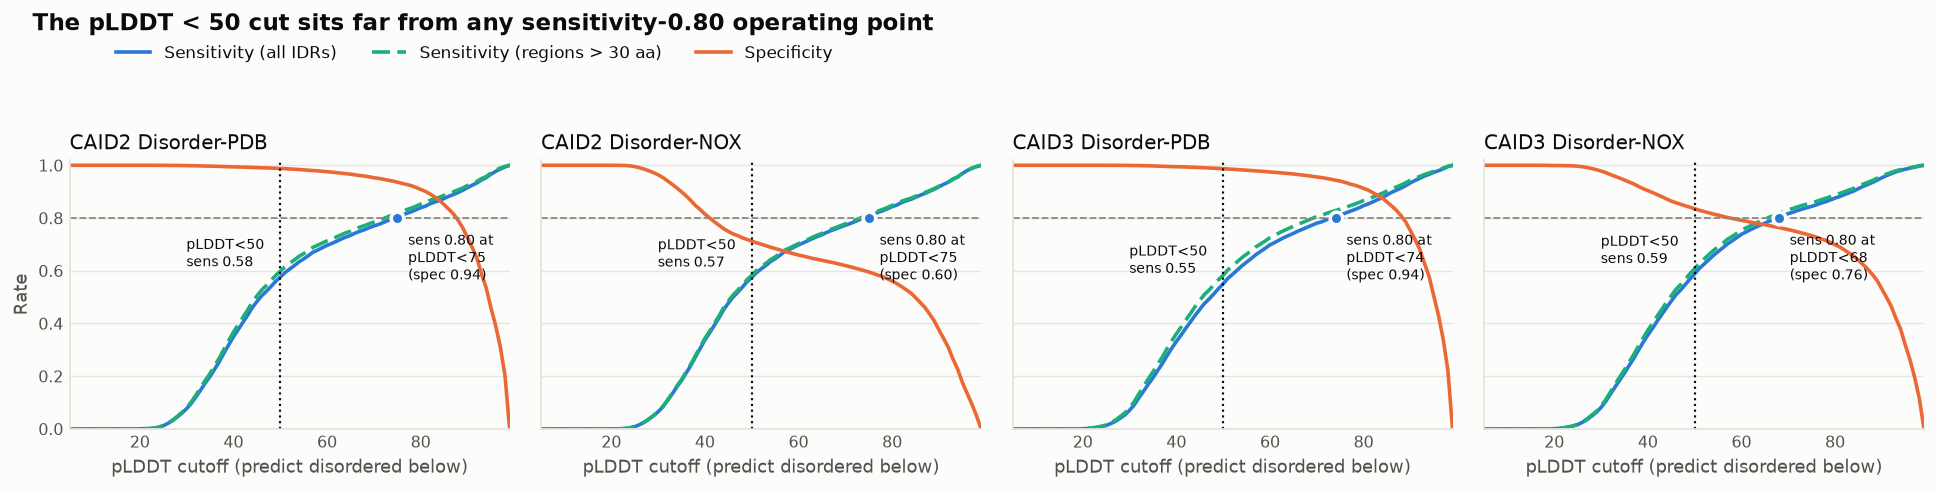
\includegraphics[width=0.95\linewidth]{figures/fig2_cutoff_sweep.png}
    \caption{Sensitivity and specificity of a \plddt cutoff as the cutoff is swept from 5 to 99.
    The vertical line marks the folk rule at 50. The AlphaFold ``very low confidence'' band was
    never calibrated against disorder annotations: on all four references the MCC-optimal
    disorder cutoff falls at \plddt 69--72, and sensitivity 0.80 is not reached until \plddt
    68--75.}
    \label{fig:sweep}
\end{figure}

\subsection{C2: specificity is decided by the negative-set convention}
\label{sec:c2}

At the identical operating point, on the same residues, with the same predictor, specificity is
$0.98$ under \dpdb and $0.67$--$0.76$ under \dnox. The claim ``specificity $<$ 0.7'' is
decisively false on both \dpdb sets ($P(\text{spec} \le 0.70) = 0.000$), consistent with the
data on \caidtwo \dnox ($0.673$, $P = 0.815$), and false on \caidthree \dnox ($0.761$,
$P = 0.032$, \ie significantly \emph{above} 0.7).

The empirical calibration in \tabref{tab:calibration} shows the mechanism. Under \dpdb,
residues in X-ray-missing segments are excluded from the negative set, so almost everything left
below \plddt 50 is a true positive and precision is 0.93--0.95. Under \dnox those same residues
become negatives, and precision collapses to 0.37--0.49 with no change whatsoever in the
predictor. Note the invariant in the last column: \textbf{\plddtrule captures 60--63\% of all
annotated disorder regardless of convention}. That is the stable, method-intrinsic quantity;
what changes is what the complement is called. Recall is the method's property, precision is the
benchmark's.

\begin{table}[t]
    \centering
    \small
    \resizebox{\textwidth}{!}{%
    \begin{tabular}{@{}lrrrrr@{}}
        \toprule
        \textbf{Reference set} & \textbf{Prevalence} & \textbf{\% res.\ \plddt$<$50} &
        $P(\text{dis.}\,|\,\plddt{<}50)$ & $P(\text{dis.}\,|\,\plddt{\ge}50)$ &
        \textbf{Disorder below 50} \\
        \midrule
        \caidtwo \dpdb   & 0.299 & 19.3 & \textbf{0.948} & 0.145 & 0.610 \\
        \caidtwo \dnox   & 0.235 & 39.6 & 0.368 & 0.148 & 0.620 \\
        \caidthree \dpdb & 0.316 & 20.4 & \textbf{0.932} & 0.159 & 0.599 \\
        \caidthree \dnox & 0.264 & 34.1 & 0.486 & 0.149 & 0.629 \\
        \bottomrule
    \end{tabular}}
    \caption{Empirical calibration of the rule. The precision of \plddtrule swings from 0.95 to
    0.37 purely with the negative-set convention, while the share of all annotated disorder that
    falls below \plddt 50 is invariant at 0.60--0.63. Reporting one convention and calling its
    specificity ``the'' specificity is the single most consequential methodological choice in
    this literature.}
    \label{tab:calibration}
\end{table}

\subsection{C4: the short-segment gap is real inside \texorpdfstring{\plddt}{pLDDT}, but dedicated predictors do not close it}
\label{sec:c4}

\para{\plddt does degrade on short regions.} \tabref{tab:strata} shows recall falling from
$0.58$--$0.61$ on regions longer than 30 aa to $0.25$--$0.43$ on regions shorter than 20 aa at
the literal cut. Calibration lifts every stratum but preserves the ordering
($0.59$--$0.65$ short versus $0.78$--$0.85$ long). Region-level detection at 50\% overlap tells
the same story: 59--81\% of short regions detected versus 80--89\% of long ones
(\tabref{tab:regiondetect}, appendix). So the premise behind \cfour --- short disorder is harder
for \plddt --- is correct.

\begin{table}[t]
    \centering
    \small
    \resizebox{\textwidth}{!}{%
    \begin{tabular}{@{}llrrlll@{}}
        \toprule
        \textbf{Reference set} & \textbf{Operating point} & \textbf{Thr.} & \textbf{Spec.} &
        \textbf{Recall $<$20 aa} & \textbf{Recall 20--30 aa} & \textbf{Recall $>$30 aa} \\
        \midrule
        \multirow{2}{*}{\caidtwo \dpdb}   & literal & 0.500 & 0.988 & 0.393 [0.324, 0.457] & 0.485 [0.379, 0.574] & 0.598 [0.537, 0.654] \\
                                          & calibrated & 0.308 & 0.956 & \textbf{0.653} [0.579, 0.721] & 0.691 [0.600, 0.777] & \textbf{0.779} [0.727, 0.827] \\
        \midrule
        \multirow{2}{*}{\caidtwo \dnox}   & literal & 0.500 & 0.712 & 0.433 [0.284, 0.570] & 0.445 [0.307, 0.567] & 0.583 [0.521, 0.651] \\
                                          & calibrated & 0.206 & 0.566 & \textbf{0.806} [0.694, 0.912] & 0.726 [0.571, 0.861] & \textbf{0.844} [0.793, 0.891] \\
        \midrule
        \multirow{2}{*}{\caidthree \dpdb} & literal & 0.500 & 0.987 & 0.331 [0.265, 0.397] & 0.407 [0.316, 0.492] & 0.583 [0.525, 0.637] \\
                                          & calibrated & 0.282 & 0.952 & \textbf{0.628} [0.555, 0.699] & 0.682 [0.585, 0.776] & \textbf{0.816} [0.769, 0.857] \\
        \midrule
        \multirow{2}{*}{\caidthree \dnox} & literal & 0.500 & 0.835 & 0.250 [0.158, 0.352] & 0.428 [0.306, 0.558] & 0.608 [0.554, 0.660] \\
                                          & calibrated & 0.272 & 0.745 & \textbf{0.587} [0.465, 0.710] & 0.726 [0.596, 0.852] & \textbf{0.846} [0.808, 0.881] \\
        \bottomrule
    \end{tabular}}
    \caption{Region-length-stratified recall of \plddt with 95\% bootstrap CIs over targets.
    Short regions are genuinely harder, at both operating points. Calibration raises recall
    everywhere by 20--35 points at a cost of 3--17 points of specificity, which is why
    comparing methods at a shared threshold is not a comparison of methods.}
    \label{tab:strata}
\end{table}

\para{But the comparative claim fails.} \tabref{tab:c4} gives the verdict. With every method
calibrated to its own MCC-optimal threshold, \emph{zero} of the 174 method\,$\times$\,dataset
comparisons is significantly better than \plddt on short segments, and the median dedicated
predictor is $1.5$--$8.7$\pp \emph{worse}. The best single result anywhere is $+6.8$\pp
(flDPnn3a on \caidthree \dnox, CI $[-0.9, +14.5]$, not significant). Under the deliberately
generous locally-flanked definition, which removes a method's global false-positive rate from
the picture entirely, the gap gets \emph{wider} rather than narrower ($-4.7$ to $-11.2$\pp).
The interaction test --- does the dedicated-predictor advantage grow specifically on short
regions, which is the substantive content of the claim --- is negative on three of four datasets
(median $-5.1$, $-4.9$, $-1.4$\pp, and $+1.7$\pp on \caidthree \dnox), with 19, 14, 17 and 7
methods showing a significantly \emph{smaller} advantage on short regions than on long ones.

\begin{table}[t]
    \centering
    \small
    \resizebox{\textwidth}{!}{%
    \begin{tabular}{@{}lrrrrrrrrr@{}}
        \toprule
        & & \multicolumn{5}{c}{\textbf{Calibrated thresholds (primary)}} & \multicolumn{3}{c}{\textbf{Shared naive 0.5 cut}} \\
        \cmidrule(lr){3-7} \cmidrule(lr){8-10}
        \textbf{Reference set} & \textbf{$n$} & \textbf{\plddt \bacc} & \textbf{$\Delta$ med.} &
        \textbf{$\Delta$ best} & \textbf{sig.\ better} & \textbf{in band} &
        \textbf{$\Delta$ med.} & \textbf{sig.\ better} & \textbf{in band} \\
        \midrule
        \caidtwo \dpdb   & 35 & 0.804 & $-8.7$ & $+0.1$ & \textbf{0} & \textbf{0} & $-0.2$ & 7 & 3 \\
        \caidtwo \dnox   & 35 & 0.686 & $-7.7$ & $+0.3$ & \textbf{0} & \textbf{0} & $+0.6$ & 3 & 1 \\
        \caidthree \dpdb & 52 & 0.790 & $-6.5$ & $+2.4$ & \textbf{0} & \textbf{0} & $+1.9$ & 21 & 6 \\
        \caidthree \dnox & 52 & 0.666 & $-1.5$ & $+6.8$ & \textbf{0} & \textbf{0} & $+7.6$ & \textbf{34} & \textbf{9} \\
        \bottomrule
    \end{tabular}}
    \caption{The claimed 10--15\% short-segment advantage of dedicated predictors is a
    calibration artefact. All deltas are percentage points of balanced accuracy on $<$20 aa
    regions relative to \plddt; ``in band'' counts methods landing inside the claimed $+10$ to
    $+15$\pp window. Left: with every method at its own MCC-optimal threshold, no method is
    significantly better and the median is worse. Right: cutting every method at 0.5 --- the
    comparison one gets by thresholding published scores --- reproduces the claim almost
    exactly on \caidthree \dnox, where 9 of 52 predictors fall inside the band and 34 are
    significantly better.}
    \label{tab:c4}
\end{table}

\para{Why the artefact arises.} At 0.5, \plddt sits at specificity 0.99 and recall 0.33 --- an
extremely conservative corner of its own ROC curve --- while a permissive predictor sits near
specificity 0.65 and recall 0.70. That is a comparison of operating points, not of methods.
Calibration moves flDPnn3a from $+19.3$\pp to $+6.8$\pp and UdonPred-combined from $+13.5$\pp to
below the median. The folk claim is a real, reproducible measurement of an artefact
(\figref{fig:short}).

\begin{figure}[t]
    \centering
    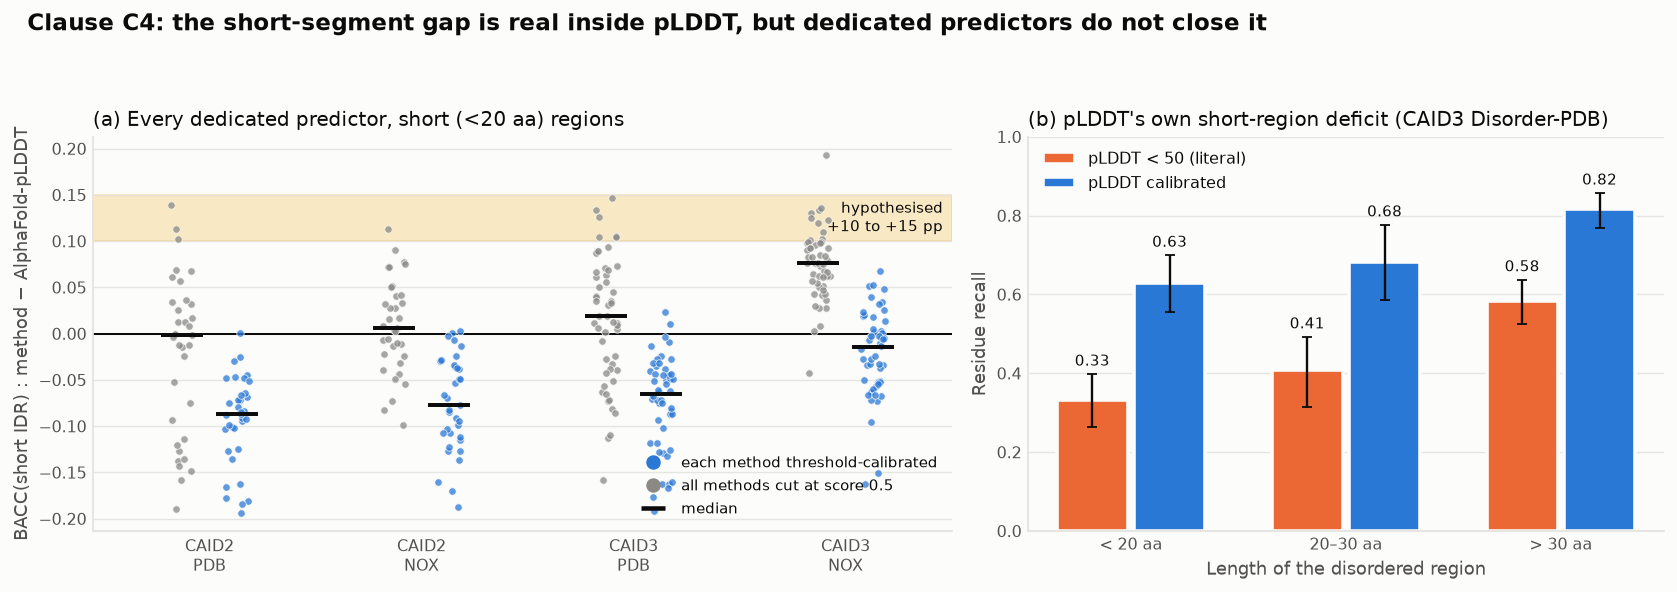
\includegraphics[width=0.95\linewidth]{figures/fig4_short_segment_claim.png}
    \caption{Per-method balanced-accuracy difference from \plddt on $<$20 aa disordered regions.
    The shaded band is the claimed $+10$ to $+15$\pp advantage. At calibrated thresholds the
    distribution sits below zero on every reference set and no method's CI clears zero; the same
    methods scored at a shared 0.5 cut populate the band. Both panels use identical residues and
    identical bootstrap resamples --- only the thresholds differ.}
    \label{fig:short}
\end{figure}

\subsection{Where \texorpdfstring{\plddt}{pLDDT} actually stands, fairly compared}
\label{sec:ranking}

Falsifying the folk claims cuts both ways. Calibrated and coverage-matched on the common target
set, \plddt is a respectable mid-pack disorder predictor (\tabref{tab:benchmark}): rank 9/37 and
11/56 on \dpdb, 16/37 and 17/56 on \dnox, comparable to IUPred3 and DISOPRED3, behind PUNCH2,
SETH-0 and the PredIDR family, ahead of flDPnn, ESpritz-D and MobiDB-lite. That is a
considerably more favourable verdict than the folk framing implies, and a considerably less
favourable one than ``\plddt $<$ 50 finds disorder'' implies. Calibration optimism is negligible:
the median gap between in-sample MCC-optimal \bacc and the $5\times2$-fold cross-validated
estimate is $0.20$--$0.66$\pp, with a maximum of $3.0$\pp across 186 method\,$\times$\,dataset
combinations, so the calibrated rankings are not an artefact of tuning on the evaluation data.

\begin{table}[t]
    \centering
    \small
    \resizebox{\textwidth}{!}{%
    \begin{tabular}{@{}lrlrlr@{}}
        \toprule
        \textbf{Reference set} & \textbf{\plddt \bacc} & \textbf{Rank} & \textbf{\plddt AUC} &
        \textbf{Best dedicated method} & \textbf{\afrsa \bacc} \\
        \midrule
        \caidtwo \dpdb   & 0.860 & 9 / 37  & 0.932 & PredIDR-long \textbf{0.887} & 0.886 \\
        \caidtwo \dnox   & 0.703 & 16 / 37 & 0.715 & SPOT-Disorder2 \textbf{0.734} & 0.713 \\
        \caidthree \dpdb & 0.871 & 11 / 56 & 0.943 & PUNCH2 \textbf{0.887} & 0.886 \\
        \caidthree \dnox & 0.789 & 17 / 56 & 0.833 & DisorderUnetLM \textbf{0.819} & 0.803 \\
        \bottomrule
    \end{tabular}}
    \caption{\plddt at its calibrated operating point against the full panel, coverage-matched.
    \plddt is mid-pack, not the outlier the folk rule's critics or its users assume; and \afrsa,
    derived from the same coordinates at no extra cost, is within a point of the best dedicated
    method on \dpdb.}
    \label{tab:benchmark}
\end{table}

\subsection{C3: \texorpdfstring{\plddt}{pLDDT} is a lossy readout of a structure that already knows better}
\label{sec:c3}

Four independent tests support the conflation mechanism.

\para{Test 1: same model, different readout.} \afrsa is the solvent accessibility of the
\emph{identical} AlphaFold2 coordinates, smoothed over a window. It beats \plddt on every
reference set: $\Delta$AUC $+0.015$ to $+0.056$ with $p \le 0.02$ throughout, and $\Delta$\bacc
$+0.017$ to $+0.044$ (\tabref{tab:readout}). This is the cleanest available test of the
conflation claim, because the structure model is held exactly fixed and only the quantity read
out of it changes. The confidence channel discards disorder-relevant information that is present
in the coordinates it is attached to.

\para{Test 2: a better folding model does not help.} AlphaFold3's \plddt is statistically
indistinguishable from AlphaFold2's on both \caidthree references ($p = 0.62$ and $0.61$), while
AlphaFold3's \emph{RSA} is significantly better ($+0.059$ AUC on \dnox, $p = 0.002$). If low
\plddt tracked genuine flexibility, a stronger folding model should sharpen it. It does not: the
gain lives in the readout, not in the model.

\begin{table}[t]
    \centering
    \small
    \resizebox{\textwidth}{!}{%
    \begin{tabular}{@{}llrrlrrr@{}}
        \toprule
        \textbf{Reference set} & \textbf{Comparison} & \textbf{$n$} & \textbf{$\Delta$AUC} &
        \textbf{95\% CI} & \textbf{$p$} & \textbf{$\Delta$\bacc} & \textbf{$p$} \\
        \midrule
        \caidtwo \dpdb   & AF2-RSA $-$ AF2-\plddt   & 299 & $\mathbf{+0.0160}$ & [$+0.0056$, $+0.0256$] & 0.002 & $+0.0263$ & 0.001 \\
        \caidtwo \dnox   & AF2-RSA $-$ AF2-\plddt   & 173 & $\mathbf{+0.0508}$ & [$+0.0201$, $+0.0894$] & 0.004 & $+0.0169$ & 0.032 \\
        \caidthree \dpdb & AF2-RSA $-$ AF2-\plddt   & 319 & $\mathbf{+0.0152}$ & [$+0.0032$, $+0.0311$] & 0.020 & $+0.0272$ & 0.001 \\
        \caidthree \dnox & AF2-RSA $-$ AF2-\plddt   & 204 & $\mathbf{+0.0561}$ & [$+0.0180$, $+0.0980$] & 0.002 & $+0.0435$ & 0.002 \\
        \midrule
        \caidthree \dpdb & AF3-\plddt $-$ AF2-\plddt & 319 & $-0.0021$ & [$-0.0102$, $+0.0082$] & 0.616 & $+0.0010$ & 0.856 \\
        \caidthree \dnox & AF3-\plddt $-$ AF2-\plddt & 204 & $+0.0072$ & [$-0.0150$, $+0.0341$] & 0.612 & $+0.0106$ & 0.356 \\
        \caidthree \dnox & AF3-RSA $-$ AF2-\plddt    & 204 & $\mathbf{+0.0585}$ & [$+0.0141$, $+0.1136$] & 0.002 & $+0.0513$ & 0.002 \\
        \bottomrule
    \end{tabular}}
    \caption{Controlled readout comparisons by paired bootstrap over targets. Changing the
    readout of a fixed AlphaFold2 model from confidence to geometry helps significantly
    everywhere; changing the folding model while keeping the confidence readout does not help at
    all.}
    \label{tab:readout}
\end{table}

\para{Test 3: residual signal inside \plddt strata.} Within the \plddt $<$ 50 stratum, \plddt
itself discriminates disorder at AUC $0.44$--$0.63$ --- at or below chance on the \dnox
references --- while RSA of the \emph{same} residues discriminates at $0.56$--$0.83$. In the
50--70 band the gap is widest (\plddt $0.56$--$0.68$ versus RSA $0.69$--$0.90$;
\tabref{tab:condinfo}, appendix). The confidence score saturates: once it has said ``not
confident'', it stops carrying information about how disordered a residue is, while the
structure still does (\figref{fig:mech}).

\para{Test 4: information overlap.} A 5-fold grouped-by-target cross-validated logistic probe on
the raw features --- an information probe, not a proposed predictor --- gives CV AUC 0.926/0.689/
0.931/0.761 for \plddt alone, 0.944/0.741/0.949/0.827 for RSA alone, and 0.949/0.743/0.956/0.822
for both. Adding \plddt on top of RSA gains at most $+0.007$ AUC and \emph{loses} $0.005$ on
\caidthree \dnox; adding RSA on top of \plddt gains $+0.023$ to $+0.065$. \plddt's disorder
information is very nearly a subset of the geometry's.

\begin{figure}[t]
    \centering
    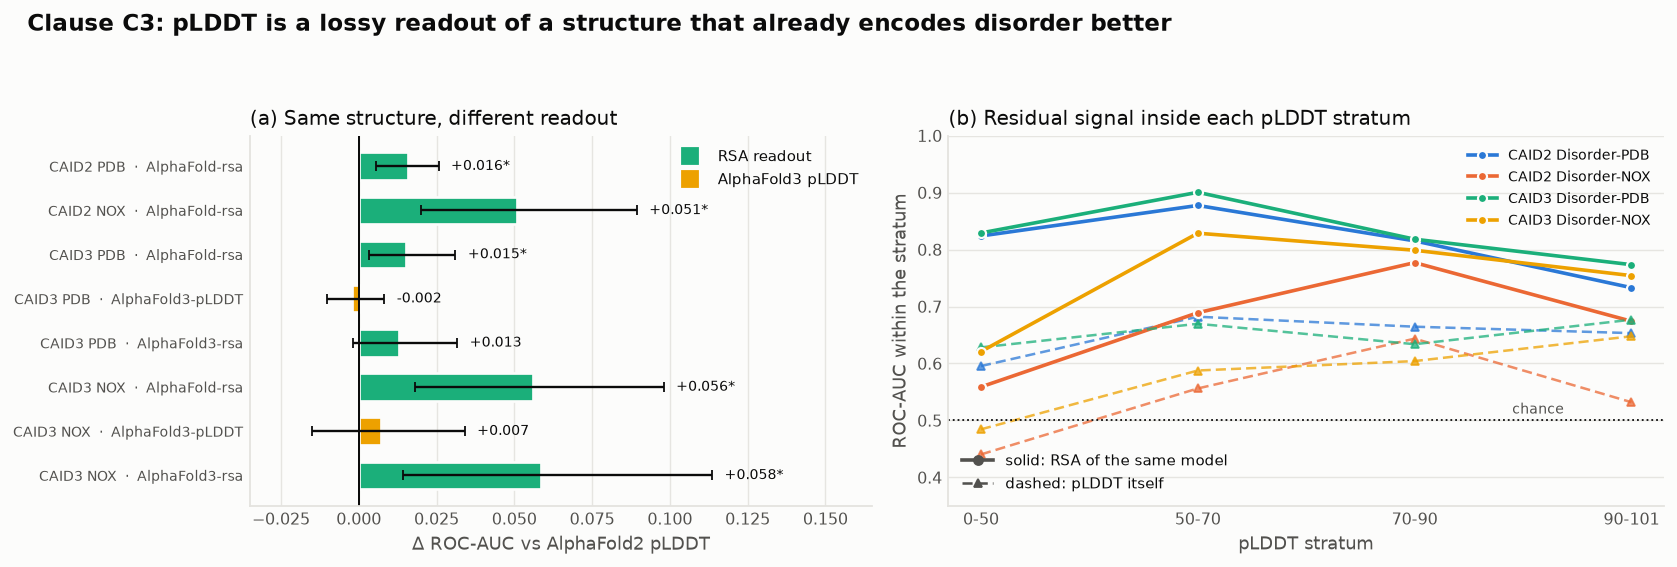
\includegraphics[width=0.95\linewidth]{figures/fig6_mechanism.png}
    \caption{The conflation mechanism. \captiona Reading solvent accessibility instead of
    confidence out of the same AlphaFold2 coordinates improves AUC on all four reference sets,
    while replacing AlphaFold2 with AlphaFold3 does not. \captionb Within \plddt strata, \plddt
    has saturated --- inside its own $<$50 band it discriminates disorder at chance level on the
    \dnox references --- while the geometry of the same model still separates disorder from
    order.}
    \label{fig:mech}
\end{figure}

\subsection{What the rule misses, structurally}
\label{sec:errors}

Decomposing the residues into true positives, false negatives, false positives and true
negatives (\tabref{tab:errorstrata}) shows what kind of disorder escapes the rule. The missed
disorder is \textbf{confidently modelled} --- mean \plddt 70--74, with 47--56\% of those residues
above \plddt 70 and 12--21\% above 90 --- and \textbf{solvent-exposed}, with mean RSA
$0.46$--$0.51$ against $0.25$--$0.31$ for true negatives, and only 17--23\% buried against
46--57\% of true negatives. It sits in shorter regions (median 110--161 aa versus 170--239 for
detected disorder) and has an intermediate amino-acid composition: detected disorder shows the
classic low-complexity signature (log$_2$ enrichment S $+0.64$, P $+0.58$, G $+0.55$, with strong
hydrophobic depletion I $-1.22$, W $-1.05$, F $-1.05$), whereas missed disorder keeps the
charged/proline enrichment (K $+0.44$, P $+0.35$, Q $+0.27$) but has no S/G enrichment
(S $-0.05$, G $-0.15$) and is only mildly hydrophobic-depleted (I $-0.37$).

\begin{table}[t]
    \centering
    \small
    \resizebox{\textwidth}{!}{%
    \begin{tabular}{@{}llrrrrr@{}}
        \toprule
        \textbf{Reference set} & \textbf{Stratum} & \textbf{$n$ residues} & \textbf{Mean \plddt} &
        \textbf{Mean RSA} & \textbf{\% buried} & \textbf{Median region len.} \\
        \midrule
        \multirow{4}{*}{\caidthree \dpdb}
          & TP (disordered, \plddt$<$50) & 18,037 & 37.0 & 0.638 & 2.7 & 170 \\
          & \textbf{FN (disordered, \plddt$\ge$50)} & 12,202 & \textbf{71.4} & \textbf{0.492} & \textbf{19.2} & \textbf{110} \\
          & FP (ordered, \plddt$<$50) & 886 & 41.4 & 0.547 & 13.9 & --- \\
          & TN (ordered, \plddt$\ge$50) & 62,840 & 91.9 & 0.255 & 56.1 & --- \\
        \midrule
        \multirow{2}{*}{\caidtwo \dpdb}
          & TP & 17,186 & 37.1 & 0.646 & 1.8 & 214 \\
          & FN & 10,428 & 73.5 & 0.463 & 23.2 & 125 \\
        \bottomrule
    \end{tabular}}
    \caption{Structural profile of the rule's error strata (2026 \afdb snapshot, Shrake--Rupley
    RSA). ``\% buried'' is the fraction with RSA $<$ 0.25. The disorder the rule misses is not
    borderline: it is confidently modelled and mostly solvent-exposed, \ie extended
    pseudostructure rather than genuinely ambiguous prediction.}
    \label{tab:errorstrata}
\end{table}

This decomposes the failure into two mechanisms with different remedies. The 17--23\% buried
fraction is \textbf{conditional folding}~\citep{alderson2023}: AlphaFold confidently builds a
folded conformation for a region that is disordered in isolation, and no confidence threshold
can recover it. The larger, exposed fraction is \textbf{pseudostructure}~\citep{richardson2025}:
AlphaFold confidently models an extended or helical conformation for a region that is genuinely
flexible. That fraction \emph{is} recoverable --- it is exactly what the RSA readout catches, and
it is why RSA beats \plddt (\figref{fig:errors}).

\begin{figure}[t]
    \centering
    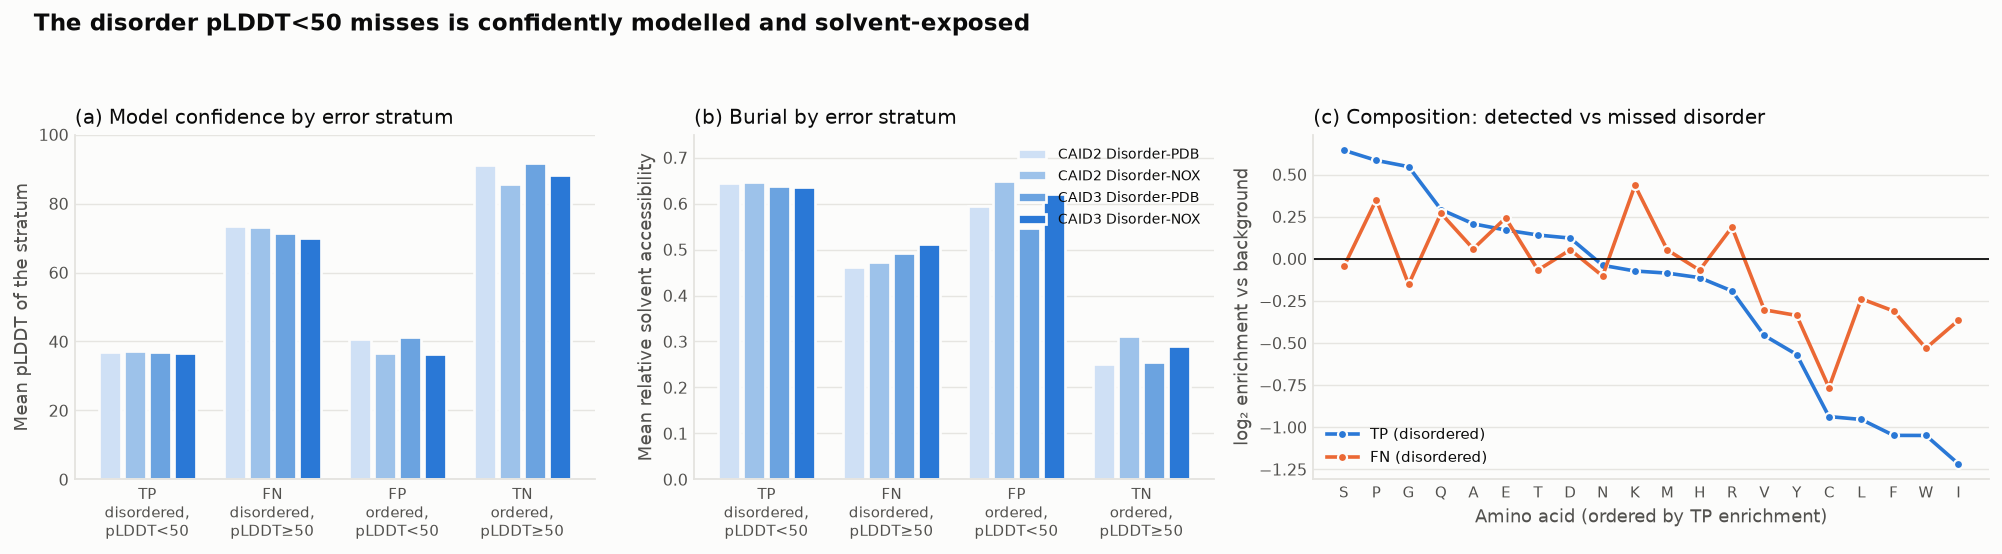
\includegraphics[width=0.95\linewidth]{figures/fig7_error_strata.png}
    \caption{What \plddtrule misses. \captiona Confidence distribution by stratum: false
    negatives are not clustered just above the cutoff but spread across the confident range.
    \captionb Solvent accessibility separates false negatives from true negatives even where
    confidence does not. \captionc Amino-acid composition places missed disorder between
    canonical low-complexity \idrs and ordered sequence, consistent with a conformation
    AlphaFold can commit to.}
    \label{fig:errors}
\end{figure}
